\chapter{Numerical Solution of Adjoint Equations}
\label{chapter-four}

This section details the derivation of the adjoint equations to be solved in
conjunction with the primal flow equations.  The primary goals of this research
are to:
\begin{enumerate}
  \item Compute sensitivities of aerodynamic and aerothermodynamic quantities to
    design variables
  \item Utilize a decoupled approach in the solution of the adjoint equations
\end{enumerate}
The cost of the solving the adjoint system of equations increases quadratically
with each additional species conservation equation, in the same manner as the
flow solver.  To mitigate this scaling, a decoupled scheme is derived to solve
the adjoint system that is consistent with the decoupled scheme used by the flow
solver.

\section{Discrete Adjoint Derivation}
\label{sec:adj-derivation}

The derivation for the discrete adjoint begins with forming the Lagrangian as
%------------------------------------------------------------------------------%
\begin{equation}
  L(\md,\mq,\mathbf{\Lambda})=f(\md,\mq)
  +\mathbf{\Lambda}^T\mr(\md,\mq)
  \label{lagrangian}
\end{equation}
%------------------------------------------------------------------------------%
where $f$ is the cost function of interest, $\mr$ is the residual of the flow
equations, $\md$ is the vector of design variables, $\mq$ is the vector of
conserved variables, and $\adjlam{}$ is the vector of Lagrange multipliers
(hereafter referred to as costate variables).  Differentiating with respect to
the design variables, $\md$, yields
%------------------------------------------------------------------------------%
\begin{equation}
  \pd{L}{\md} = 
  \pd{f}{\md} + \left[ \pd{\mq}{\md} \right]^T \left\{ 
    \pd{f}{\mq} + \left[ \rdiff{}{\mq} \right]^T \adjlam{}
  \right\}
  + \left[ \rdiff{}{\md} \right]^T \adjlam{}
  \label{dL}
\end{equation}
%------------------------------------------------------------------------------%
To eliminate the dependence of conserved variables, $\mq$, on the design
variables, we solve the adjoint equation
%------------------------------------------------------------------------------%
\begin{equation}
  \bigg[\pd{\mr}{\mq}\bigg]^T\mathbf{\Lambda} = -\pd{f}{\mq}
  \label{adjoint-main}
\end{equation}
%------------------------------------------------------------------------------%
\eref{dL} can ultimately be used in error estimation and sensitivity analysis
for design optimization.  With the second term in \eref{dL} eliminated, the
derivative of the Lagrangian becomes
%------------------------------------------------------------------------------%
\begin{equation}
  \pd{L}{\md}=
  \pd{f}{\md} + \left[ \rdiff{}{\md} \right]^T \adjlam{}
  \label{obj-function}
\end{equation}
%------------------------------------------------------------------------------%
The sensitivity of the objective function to the design parameters can be used
by a non-linear optimizer to determine an optimal set of design variables,
$\md^*$. This optimization can be done using {\bf SNOPT\cite{snopt-manual}},
{\bf KSOPT\cite{KSOPT}}, or {\bf NPSOL\cite{npsol-manual}} in FUN3D, as well as
a host of other non-linear optimizers.


\section{Fully Coupled Adjoint Formulation}
\label{sec:fully-coupled-adj}

For the fully coupled system in \eref{fc-global}, the adjoint system from
\eref{adjoint-main} is written as
%------------------------------------------------------------------------------%
\begin{equation}
  \rtdiff{\mU}{\mU} \adjlam{\mU} = - \pd{f}{\mU}
  \label{fc-adjoint-system}
\end{equation}
%------------------------------------------------------------------------------%
where $\adjlam{\mU}$ is the vector of costate variables associated with the
fully coupled flow solver equation set.  It is important to note that the
linearizations in $\rtdiff{\mU}{\mU}$ from \eref{fc-adjoint-system} must be
exact, whereas the Jacobian used by the flow solver in \eref{fc-adjoint-system}
can contain approximations.  \eref{fc-adjoint-system} is a linear system of
equations, and can be solved via a linear solver such as GMRES
\cite{saad1986gmres}; however, Nielsen \cite{nielsenPhD} found that
time-marching the FUN3D discrete adjoint linear system with the same
point-implicit scheme as the FUN3D flow solver was more robust, and solved
systems where GMRES tended to stall.  The time marching algorithm also has the
benefit of reusing the approximate Jacobians from the flow solver, transforming
\eref{fc-adjoint-system} into
%------------------------------------------------------------------------------%
\begin{equation}
  \left(
    \frac{\vol}{\Delta t} \mi + \druduapprox
  \right)^{\mathsmaller T} \Delta \adjlam{\mU}
  =
  -\left(\pd{\ru{}}{\mU}^{\mathsmaller T}\adjlam{\mU}^n + \pd{f}{\mU} \right)
  \label{fc-adj-time}
\end{equation}
%------------------------------------------------------------------------------%
Using the same linear solver as the fully coupled flow solver to solve
\eref{fc-adj-time} results in the same quadratic scaling in cost and memory that
the fully coupled flow solver scheme suffered.

\section{Block Jacobi Adjoint Decoupling}
\label{block-jacobi-decoupling}

It is possible to decouple the adjoint equations in a fashion similar to that
done to the primal flow equations.  This begins by recognizing that the
decoupled scheme can actually also be solved as a fully-coupled system of
equations that involves the following change of variables and change of
equations
%------------------------------------------------------------------------------%
\begin{equation}
  \mU = \begin{pmatrix}
    \rho_1 \\
    \vdots \\
    \rho_{ns} \\
    \rho \vu \\
    \rho E
  \end{pmatrix}
  \rightarrow
  \mv = \begin{pmatrix}
    c_1 \\
    \vdots \\
    c_{ns} \\
    \rho \\
    \rho \vu \\
    \rho E
  \end{pmatrix}
  \label{u-v-vars}
\end{equation}
%------------------------------------------------------------------------------%
%------------------------------------------------------------------------------%
\begin{equation}
  \ru{} =
  \begin{pmatrix}
    \res{\rho_1} \\
    \vdots \\
    \res{\rho_{N_s}} \\
    \res{\rho \vu} \\
    \res{\rho E}
  \end{pmatrix}
  \rightarrow
  \rv{} =
  \begin{pmatrix}
    \res{\rho_1} - c_1 \resrho \\
    \vdots \\
    \res{\rho_{N_s}} - c_{N_s} \resrho \\
    \resrho \\
    \res{\rho \vu} \\
    \res{\rho E}
  \end{pmatrix}
  \label{fc-to-dc-res}
\end{equation}
%------------------------------------------------------------------------------%
Exactly linearizing the equation set $\rv{}$ for the variable set $\mv$ at a
single point results in the Jacobian
%------------------------------------------------------------------------------%
\begin{gather}
  \drvdv = 
  \begin{pmatrix}
    \tpdiff{\rho_1}{c_1}      & \dots  & \tpdiff{\rho_1}{c_{N_s}}     & \tpdiff{\rho_1}{\rho}     & \tpdiff{\rho_1}{\rho \vu}     &  \tpdiff{\rho_1}{\rho E}  \\
    \vdots                    & \ddots & \vdots                       & \vdots                    & \vdots                        & \vdots                    \\
    \tpdiff{\rho_{N_s}}{c_1}  & \dots  & \tpdiff{\rho_{N_s}}{c_{N_s}} & \tpdiff{\rho_{N_s}}{\rho} & \tpdiff{\rho_{N_s}}{\rho \vu} &  \tpdiff{\rho_{N_s}}{\rho E}    \\
    \tdiff{\rho}{c_1}         & \dots  & \tdiff{\rho}{c_{N_s}}        & \tdiff{\rho}{\rho}        & \tdiff{\rho}{\rho \vu}        &  \tdiff{\rho}{\rho E}     \\
    \tdiff{\rho \vu}{c_1}     & \dots  & \tdiff{\rho \vu}{c_{N_s}}    & \tdiff{\rho \vu}{\rho}    & \tdiff{\rho \vu}{\rho \vu}    &  \tdiff{\rho \vu}{\rho E} \\
    \tdiff{\rho E}{c_1}       & \dots  & \tdiff{\rho E}{c_{N_s}}      & \tdiff{\rho E}{\rho}      & \tdiff{\rho E}{\rho \vu}      &  \tdiff{\rho E}{\rho E}
  \end{pmatrix}
  \label{dc-full-system}
\end{gather}
%------------------------------------------------------------------------------%
The same solution method as the decoupled flow solver can be used to time march
the adjoint linear system of equations to the solution, solving the following
systems
%------------------------------------------------------------------------------%
\begin{gather}
  \left(
  \frac{\rho \vol}{\Delta t} \mi + \pd{\mathbf{\tilde{R}_{\Vhat}}}{\Vhat}
  \right)^{\mathsmaller T} \Delta \adjlam{\Vhat}
  =
  -\left(\pd{\rv{}}{\Vhat}^{\mathsmaller T}\adjlam{\mv}^n + \pd{f}{\Vhat} \right)
  \label{dc-species-adj-time} \\
  \left(
  \frac{\vol}{\Delta t} \mi + \pd{\mathbf{\tilde{R}_{\Up}}}{\Up}
  \right)^{\mathsmaller T} \Delta \adjlam{\Up}
  =
  -\left(\pd{\rv{}}{\Up}^{\mathsmaller T}\adjlam{\mv}^n + \pd{f}{\Up} \right)
  \label{dc-mixture-adj-time}
\end{gather}
%------------------------------------------------------------------------------%
where $\adjlam{\mv}$ is the vector of costate variables associated with the
equation set $\rv{}$ in \eref{fc-to-dc-res}, and is comprised of $\adjlam{\Vhat}$
(species continuity equations) and $\adjlam{\Up}$.  If a block Jacobi scheme is
used, the order in which \erefs{dc-species-adj-time}{dc-mixture-adj-time} are
solved is inconsequential, since no information in the costate variable vector,
$\adjlam{\mv}$, is passed between these two systems.

While \erefs{dc-species-adj-time}{dc-mixture-adj-time}
recovers the same benefits in linear solver that were afforded the decoupled
flow solver scheme, namely linear scaling in cost with additional species
continuity equations, \eref{dc-full-system} shows that forming
$\drvdv$ explicitly requires more work than forming
$\drudu$.  There is also a serious concern in the development time
required to implement and maintain both exact Jacobians, $\drvdv$ and $\drudu$.
An attractive alternative to explicitly forming $\drvdv$ is to apply a series of
matrix transformations to $\drudu$ in order to recover $\drvdv$.  It is possible
to left and right precondition \eref{fc-adjoint-system} to form the RHS of
\erefs{dc-species-adj-time}{dc-mixture-adj-time}
%------------------------------------------------------------------------------%
\begin{gather}
  \underbrace{
    \left( \pd{\mU}{\mv} \right)^{T}
  }_\text{Left Preconditioner}
  \left( \pd{\ru{}}{\mU} \right)^{T}
  \underbrace{
    \left( \pd{\rv{}}{\ru{}} \right)^{T}
  }_\text{Right Preconditioner}
  \adjlam{\mv}
  = 
  -
  \underbrace{
    \left( \pd{\mU}{\mv} \right)^{T}
  }_\text{Left Preconditioner}
  \pd{f}{\mU} 
  \label{fc-to-dc-adj} \\[12pt]
  \adjlam{\mU} = \left( \pd{\rv{}}{\ru{}} \right)^{T} \adjlam{\mv}
  \label{right-precond}
\end{gather}
%------------------------------------------------------------------------------%
The derivation of the transformation matrices, $\pd{\mU}{\mv}$ and
$\pd{\rv{}}{\ru{}}$, are included in \aref{change-of-var-section} and
\aref{sec:change-of-equations}, respectively.  Using
\erefs{fc-to-dc-adj}{right-precond}, it is possible to rewrite
\eref{dc-species-adj-time} and \eref{dc-mixture-adj-time} in terms of the fully
coupled system linearizations and costate variables
%------------------------------------------------------------------------------%
\begin{gather}
  \left(
  \frac{\rho \vol}{\Delta t} \mi + \pd{\mathbf{\tilde{R}_{\Vhat}}}{\Vhat}
  \right)^{\mathsmaller T} \Delta \adjlam{\Vhat}
  =
  - \left( \pd{\mU}{\Vhat} \right)^{\mathsmaller T}
  \left(\pd{\ru{}}{\mU}^{\mathsmaller T}\adjlam{\mU}^n + \pd{f}{\mU} \right)
  \label{dc-fc-species-adj-time} \\
  \left(
  \frac{\vol}{\Delta t} \mi + \pd{\mathbf{\tilde{R}_{\Up}}}{\Up}
  \right)^{\mathsmaller T} \Delta \adjlam{\Up}
  =
  - \left( \pd{\mU}{\Up} \right)^{\mathsmaller T}
  \left(\pd{\ru{}}{\mU}^{\mathsmaller T}\adjlam{\mU}^n + \pd{f}{\mU} \right)
  \label{dc-fc-mixture-adj-time}
\end{gather}
%------------------------------------------------------------------------------%
\erefs{dc-fc-species-adj-time}{dc-fc-mixture-adj-time} effectively utilize the
fully coupled scheme linearizations and pre-processes them before the linear
solver to make them consistent with the approximations used in the decoupled
flow solve Jacobians.  This is very efficient from an implementation standpoint,
as the infrastructure required to compute the exact linearizations of the
second-order reconstruction scheme is extremely involved.  The only change
necessary on the RHS of decoupled adjoint solver systems is accomplished by
looping over the adjoint residual vector and the costate variable vector to
apply the necessary changes.  For the LHS, the Jacobians can be directly reused
from the flow solver routines, and only high-level changes are necessary to
facilitate the transpose operations.


\section{Higher-order Reconstruction Linearizations}
\label{sec:higher-order-linearizations}

The reconstruction scheme detailed in \sref{sec:2nd-order-reconstruction} must
be exactly linearized in the adjoint solver to achieve correct sensitivity
derivatives. The adjoint uses a frozen flux limiter, for purposes that will be
discussed in a later section, and is therefore held as constant in the
linearization computations.  All gradient information in \eref{u-muscl},
$\pd{q_{1,2}}{x}$, $\pd{q_{1,2}}{y}$, and $\pd{q_{1,2}}{z}$, are computed using
least-squares.  For the example stencil shown in \fref{fig:lsq-gradients} this
is effectively computed as
%------------------------------------------------------------------------------%
\begin{equation}
  \begin{aligned}
    \pd{q}{x} &= \sum_{i=1}^{5}{W_{x,i}\left( q_i - q_0 \right)} \\
    \pd{q}{y} &= \sum_{i=1}^{5}{W_{y,i}\left( q_i - q_0 \right)} \\
    \pd{q}{z} &= \sum_{i=1}^{5}{W_{z,i}\left( q_i - q_0 \right)}
  \end{aligned}
  \label{grad-construction}
\end{equation}
%------------------------------------------------------------------------------%
where the $z$ direction would come from geometry out of the page.
%------------------------------------------------------------------------------%
\begin{figure}[h]
  \centering
  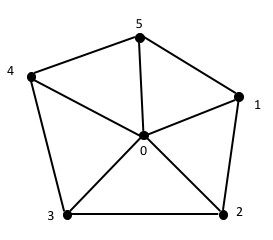
\includegraphics[width=0.5\textwidth]{figures/stencil.png}
  \caption{Example stencil for least-squares gradient evaluation.}
  \label{fig:lsq-gradients}
\end{figure}
%------------------------------------------------------------------------------%
In practice, the higher order linearizations can be managed easily by
constructing a list of neighboring nodes for each node.  By the chain rule the
linearization of the residual, $\mr$, is then evaluated in two parts
%------------------------------------------------------------------------------%
\begin{equation}
  \pd{\vR\left(\mU^*\left( \mU \right) \right)}{\mU} = 
  \pd{\vR}{\mU} + \pd{\vR}{\mU^{*}}\pd{\mU^*}{\mU}
  \label{residual-high-low}
\end{equation}
%------------------------------------------------------------------------------%
where $\mU$ are the conserved variables at each node, and $\mU^*$ are the higher
order terms computed in the U-MUSCL reconstruction; therefore, after computing
the exact first-order Jacobian of the Roe FDS scheme, $\pd{\vR}{\mU}$, the
higher order linearizations are computed by making a circuit around each node to
pick up the contributions from the least squares gradient computation.  For the
example stencil in \fref{fig:lsq-gradients}, the contribution to the residual
from looping around node 0 would be
%------------------------------------------------------------------------------%
\begin{equation}
  \pd{\vR_0}{\mU^*}\pd{\mU^*}{\mU} = \pd{\vR_0}{\mU^*} \left[\sum_{i=1}^5{(1-\kappa)
  \left( -W_{x,i}dx - W_{y,i}dy - W_{z,i}dz \right) \pd{q_0}{\mU}}\right]
  \label{ho-linearization}
\end{equation}
%------------------------------------------------------------------------------%
An important point that this illustrates is that the form of the higher order
linearizations does not change significantly based on the primitive variable
vector $q$, only affecting the primitive to conserved variable Jacobian,
$\pd{q_0}{\mU}$, which is easily computed.  This is a powerful telescoping
property of the reconstruction scheme from \sref{sec:2nd-order-reconstruction},
and it significantly decreases the complexity of the code required to implement
the second order term linearizations.  The downside of looping around each node
is the high number of cache misses, as the data structures in FUN3D are not
conducive to co-locating memory based on stencil.  This results in the
evaluation of the second order linearizations being the dominant computational
cost in the adjoint solver.

\section{Memory and Computational Cost of Exact Second Order Linearizations}
\label{sec:2nd-order-mem-cost}

As shown in \sref{sec:higher-order-linearizations}, the second order
reconstruction results in an extended stencil.  This significantly decreases the
sparsity of the Jacobian, since the linearizations at a node must now include
the neighbors of its nearest neighbors.  The cost of computing these
linearizations can quickly dominate other costs of the adjoint, but can be
significantly mitigated if the linearizations of second order Jacobian are
stored.  This essentially trades all the memory in the simulation for
computational speed, and may not be possible for large mesh sizes.  Since all of
the linearizations in the second order Jacobian must be exact, the memory saving
approximations of the decoupled scheme can only be applied to the LHS Jacobians
in \erefs{dc-fc-species-adj-time}{dc-fc-mixture-adj-time}.  This last point
makes the quadratic scaling of memory required with the number of species a
significant concern of the adjoint.  The savings provided by the decoupled
scheme become a very significant benefit in cases involving many species, since
the memory freed by the sparsity on the LHS of
\erefs{dc-fc-species-adj-time}{dc-fc-mixture-adj-time} can be used by the RHS
linearizations to increase the computational efficiency of the adjoint solver.
